\documentclass{beamer}

\usepackage[latin1]{inputenc}
\usepackage{graphicx}
\usepackage{amsmath,amssymb,amsthm}
\usepackage[mathscr]{eucal}
\usepackage{textcomp}
\usepackage{subfig}
\usepackage{epsfig}
\usepackage{multirow}
\usepackage{hhline}
\usepackage{bm}
\usepackage{makecell}

\renewcommand\theadalign{bc}
\renewcommand\theadfont{\bfseries}
\renewcommand\theadgape{\Gape[4pt]}
\renewcommand\cellgape{\Gape[4pt]}

\usefonttheme[onlymath]{serif}

\beamertemplatetextbibitems

%% Table of contents at beginning of each section
\AtBeginSection[]
{
  \begin{frame}<beamer>
    % \frametitle{Section \thesection}
    \tableofcontents[currentsection]
  \end{frame}
}

%% Current 
\usetheme{Frankfurt}
\usecolortheme{seahorse}
\setbeamertemplate{footline}[page number]
% \usecolortheme{albatross} % <-- To view white background images

% \usetheme{Boadilla}
% \usecolortheme{seahorse}

%% Footnote for Figures
\newcommand\blfootnote[1]{%
   \begingroup
   \renewcommand\thefootnote{}\footnote{#1}%
   \addtocounter{footnote}{-1}%
   \endgroup
}

\usepackage[latin1]{inputenc}

\title[Tensor-Based Signal Processing]{Noninvasive Assessment of Atrial Fibrillation Complexity Using Tensor Decomposition Techniques} 
\author[Lucas Abdalah]{\textbf{Lucas Abdalah}, Pedro M. R. de Oliveira, Walter Freitas Jr, Vicente Zarzoso}
\date{Oct 11{\textsuperscript{th}}, 2022}

\begin{document}
%% ------------------------- Title --------------------------------------------
	\begin{frame}
		\begin{figure}[!htb]
			\centering
			
\includegraphics[scale=0.055]{figures/UCA_logo} 
			% 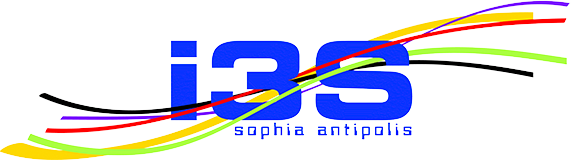
\includegraphics[scale=0.150]{figures/I3S_logo} 
			% 
\includegraphics[scale=0.025]{figures/CNRS_logo.png} 
			
\includegraphics[scale=0.130]{figures/UFC_logo.png}
		\end{figure}
		% \vspace{-0.4cm}

		\titlepage
	\end{frame}

%% ------------------------- Introduction -------------------------------------
\section{Introduction} 
	
	\begin{frame}{Atrial Fibrillation}	
		
		\begin{itemize}
			\item Atrial Fibrillation (AF) is the most common sustained cardiac arrhythmia encountered in clinical practice.
			\begin{itemize}
				\item  In the EU, the number of adults with AF will double from 2010 to 2060\footnote{Krijthe \textit{et al}., ``Projections on the number of individuals with atrial fibrillation in the European Union, from 2000 to 2060,'' \textit{Eur Heart J}. 2013.}.
			\end{itemize}
		\end{itemize}
		\begin{figure}
			\centering
			\includegraphics[scale=0.2]{figures/AF_ECG-eps-converted-to.pdf}
		\end{figure}
		\vspace{-0.8in}	
		\begin{itemize}
			\item The complex electrophysiological mechanisms underlying AF are not completely understood.
		\end{itemize}
	\end{frame}

	\begin{frame}{Step-wise Catheter Ablation (CA)}
		
		\begin{figure}[h]
			\centering
			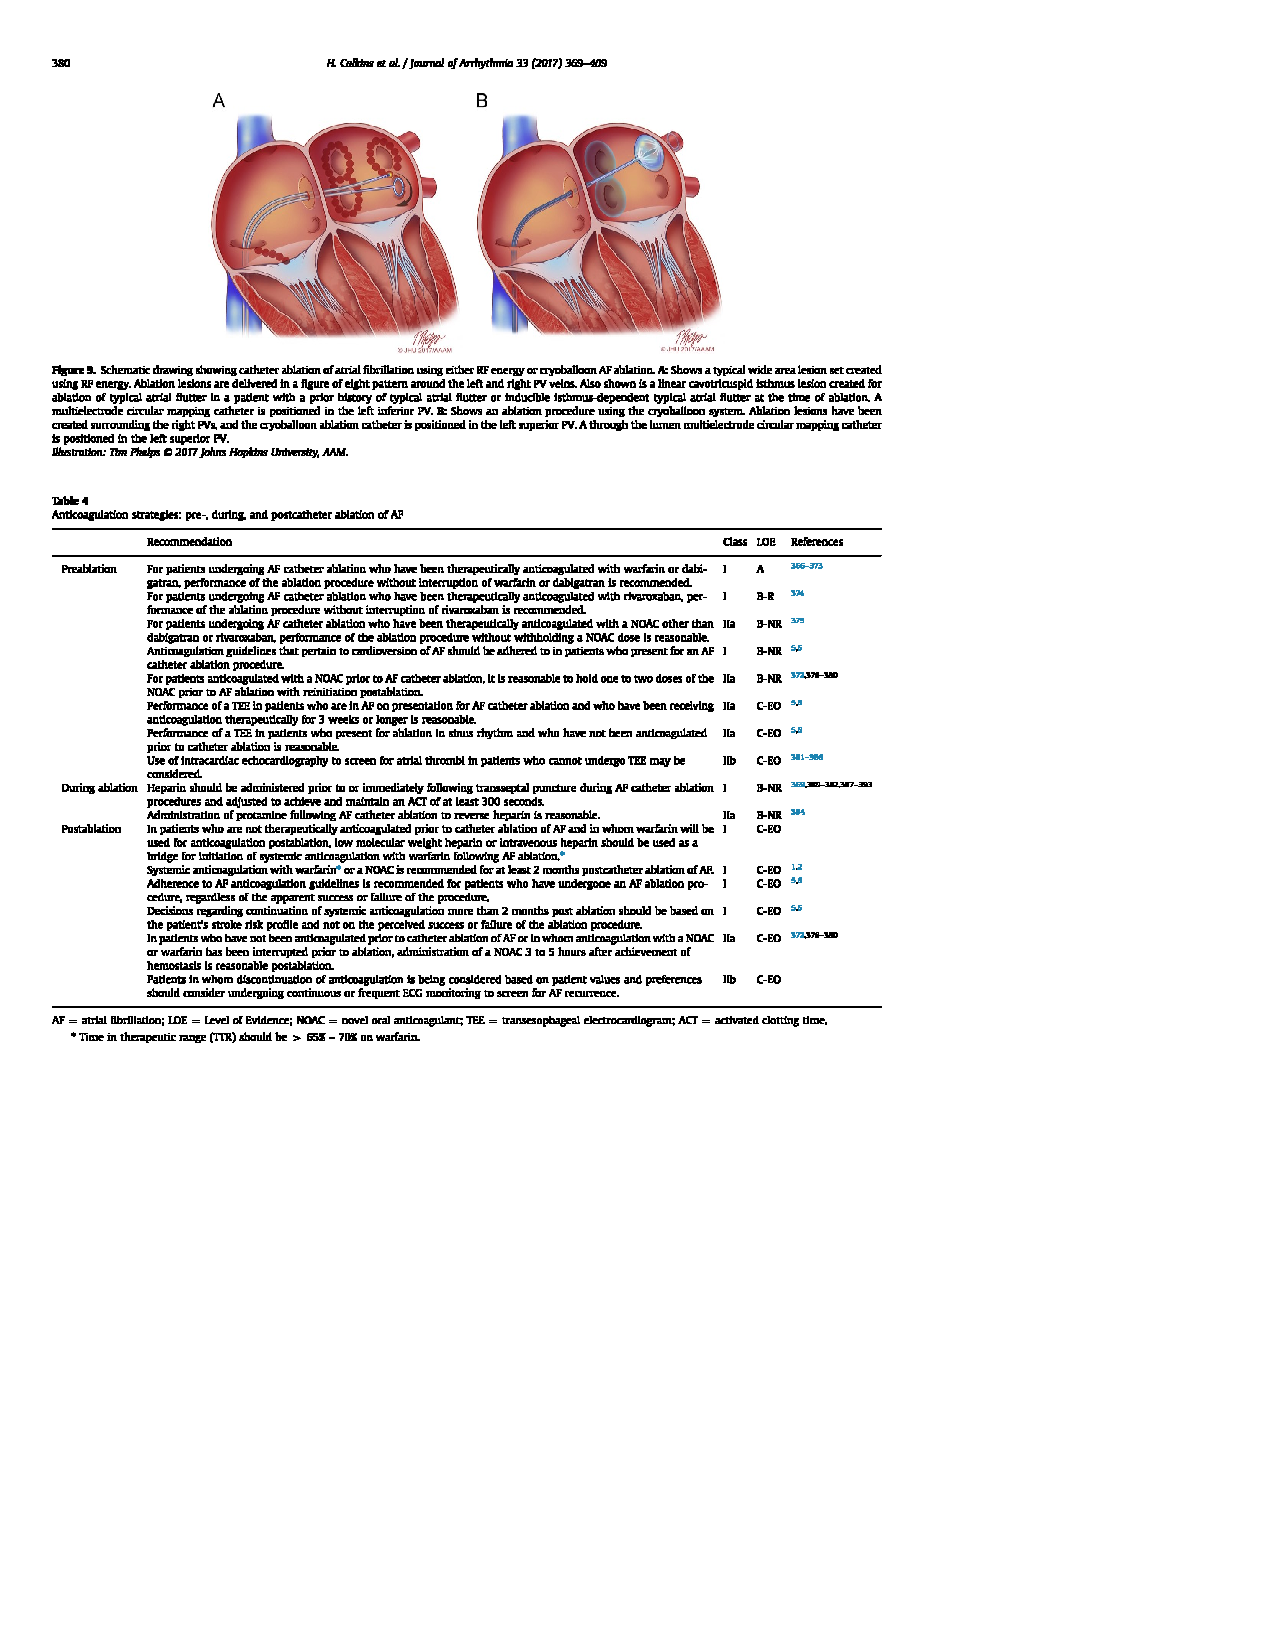
\includegraphics[scale=1.2,clip=true,trim={3.55cm 21.95cm 13.8cm 2.0cm}]{figures/CA_figure.pdf}
		\end{figure}
		\blfootnote{Figure from Tim Helps $^{\text{\tiny{\copyright}}}$ 2017 Johns Hopkins University, AAM}
		\vspace{-0.8cm}
		\begin{itemize}
			\item Noninvasive techniques to assess AF electrophysiological complexity can help guide step-wise CA in real time.
			\begin{itemize}
				\item Impact of pulmonary vein isolation (PVI) and other widely used techniques on atrial activity (AA) complexity.
			\end{itemize}
		\end{itemize}
	\end{frame}

	\begin{frame}{BSS Model}
	
		The ECG data matrix can be modeled as:
		\begin{equation}
			\textbf{Y} = \textbf{MS} \in \mathbb{R}^{K \times N} \; ,
		\end{equation}
		where ${\textbf{M}} \in {\mathbb{R}}^{K \times R}$ is a mixing matrix and $\textbf{S} \in {\mathbb{R}}^{R \times N}$ is the source matrix.	
		% \vspace{-0.4cm}
		\begin{figure}[htb]
			\centering
			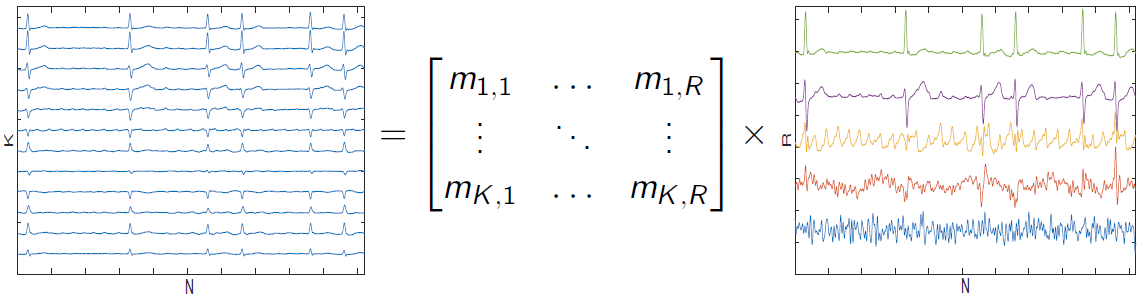
\includegraphics[scale=0.47]{figures/bss_fig.png}
		\end{figure}
	\end{frame}
		
%% ------------------------- Methods ------------------------------------------
\section{Methods}

	\begin{frame}{Matrix Approach}
		\begin{itemize}
			\item Nondipolar Component Index (NDI)\footnote{M. Meo et. al, ``Noninvasive assessment of atrial fibrillation complexity in relation to ablation characteristics and outcome,'' \textit{Frontiers in Physiology}, 2018.}
			\begin{itemize}
				\item PCA applied to TQ Intervals
				\item AA is represented by the 3D subspace spanned by its first 3 PCs
			\end{itemize}
		\end{itemize}
		\begin{figure}[htb]
			\centering
			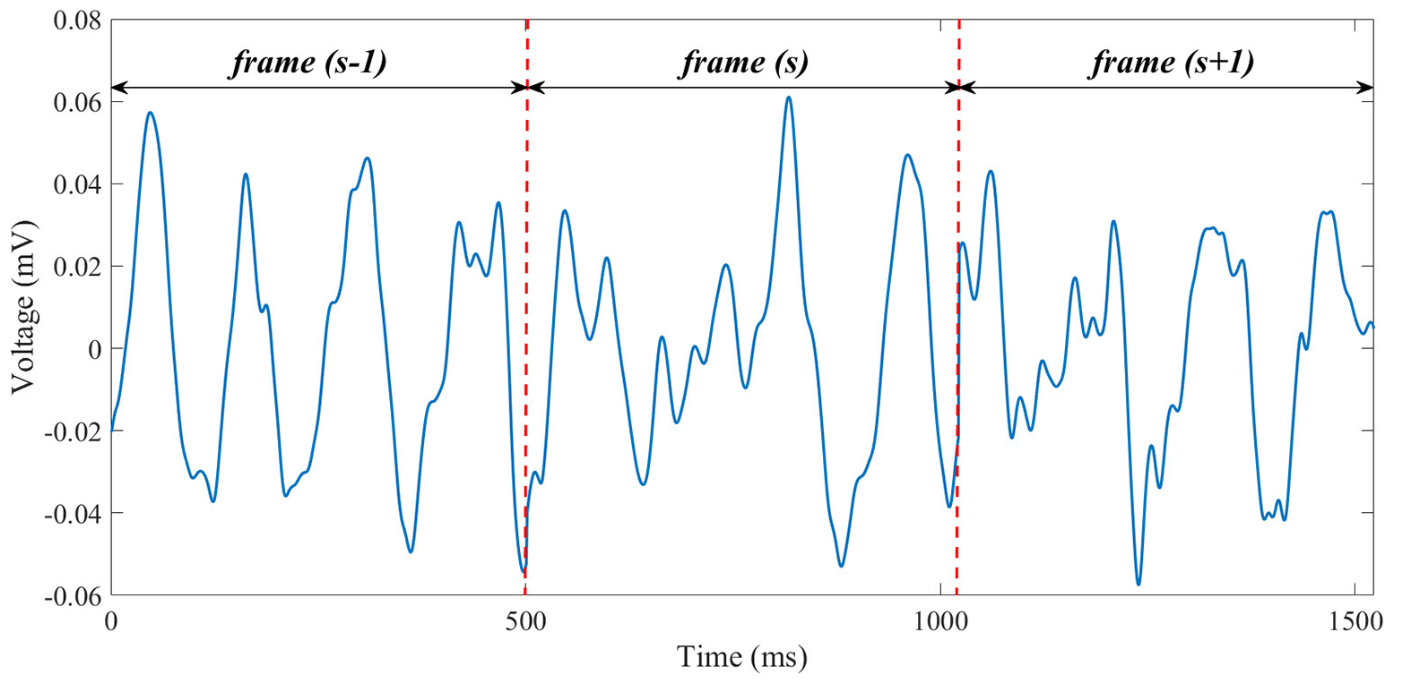
\includegraphics[scale=0.17]{figures/MEO-NDI-TQ-Concatenation.png}
		\end{figure}
		\blfootnote{Figure from M. Meo et al., 2018.}
	\end{frame}

	\begin{frame}{Nondipolar Component Index (NDI)}
		
		\begin{itemize}
				\item Compute PCA on the preprocessed ECG
		\end{itemize}

		\begin{equation}
			{\bf Y}_{TQ} = {\bf U} {\bf \Sigma} {\bf V}^T
		\end{equation}

		\begin{itemize}
			\item The proportion of power not explained by the 3 dominant PCs
	\end{itemize}

		\begin{equation}
			\text{NDI} = 1 - \frac{\sum_{l=1}^{3} \sigma_{l}^2}{\sum_{l=1}^{L} \sigma_{l}^2}.
		\end{equation}

	\end{frame}

	\begin{frame}{Tensor Approach}
		
		\begin{itemize}
			\item The ECG data can be modeled as a 3rd-order tensor ${\mathcal{Y}}$ via row-Hankelization.
			\begin{itemize}
				\item Tensor decompositions factorize data as a sum of simpler tensors.
			\end{itemize}
		\end{itemize}
		\vspace{-0.7cm}
		\begin{figure}[htb]
			\centering
			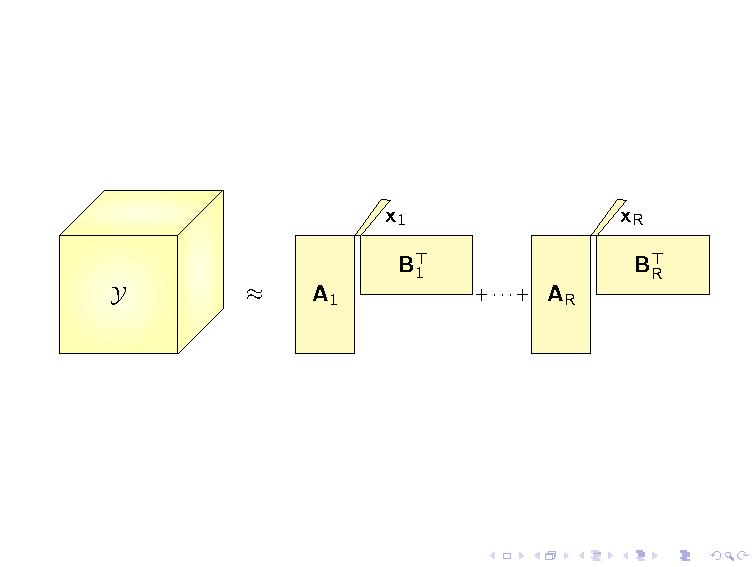
\includegraphics[scale=0.8,clip=true,trim={0.8cm 6.5cm 0.6cm 6.2cm}]{figures/tikz_BTDY.pdf}
		\end{figure}
		\vspace{2.3cm}
		\begin{itemize}
			\item Block Term Tensor Decomposition (BTD) based on Hankel structure\footnote{De Lathauwer, ``Blind separation of exponential polynomials and the decomposition of a tensor in rank-($L_{r}$,$L_{r}$,1) terms,'' \textit{SIAM J. Matrix Anal. Appl.}, 2011.}.
		\end{itemize}
	\end{frame}
		
	\begin{frame}{BTD-Hankel Model}
	
		\begin{block}{Low-rank Hankel Structure}
			\begin{itemize}
				\item The signal $s(n)$ is represented by an all-pole model~(\ref{eq:source_model})
        		\item A Hankel matrix has a rank equal to the number of poles ($L$)
		    \end{itemize}
		\end{block}
		\vspace{-10pt}
		\begin{equation}
			s(n) = \sum_{l = 1}^{L} c_{l} z_{l}^{n}, \quad 0\leq n \leq N-1  \label{eq:source_model}
		\end{equation}
		\vspace{-10pt}
		\begin{figure}[htb]
			\centering
			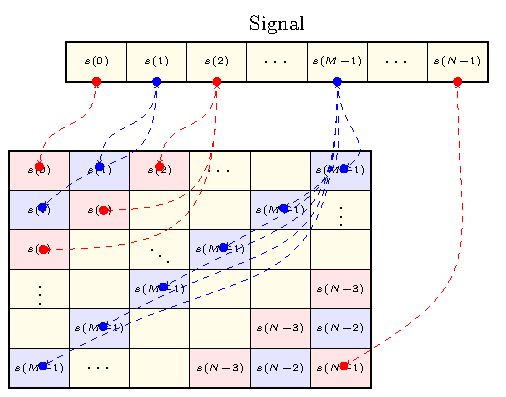
\includegraphics[scale=0.64]{figures/tikz_mapHankel_NOTATION.pdf}
		\end{figure}
	\end{frame}

	\begin{frame}{Tensor Approach}
		
		\vspace{-3.5cm}
		\begin{itemize}
			\item Stack each Hankel matrix in the 3rd-mode of the tensor $\mathcal{Y}$.
		\end{itemize}
		
		\vspace{3.0cm}
		\begin{figure}[!ht]
			\centering
			\vspace{-3.5cm}
			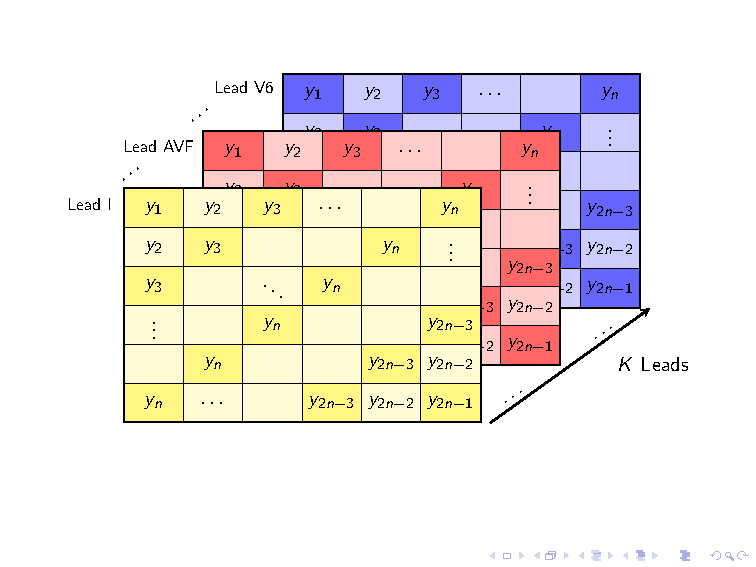
\includegraphics[scale=1.0,trim={1.0cm 8.5cm 1.0cm 7.3cm},clip=true]{figures/tikz_tensorHankel.pdf}
		\end{figure}
	\end{frame}

	\begin{frame}{BTD Approach}
		
		\vspace{-0.7cm}
		\begin{figure}[htb]
			\centering
			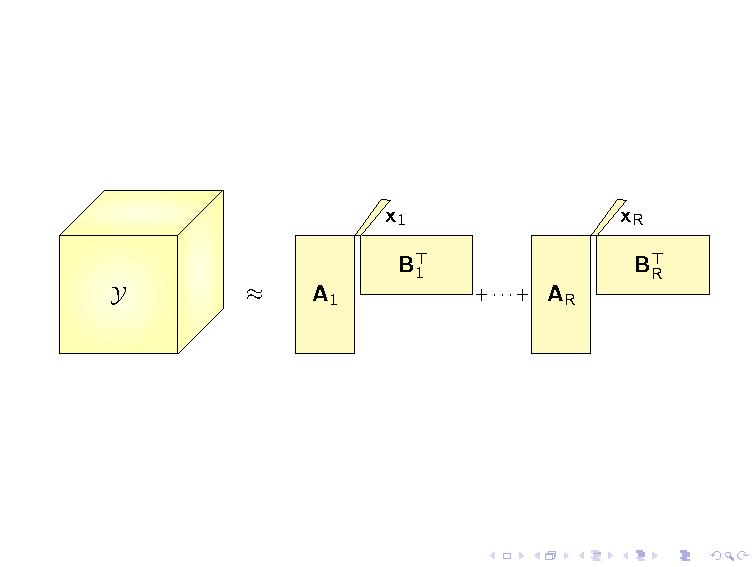
\includegraphics[scale=1.0,clip=true,trim={0.8cm 6.5cm 0.6cm 6.2cm}]{figures/tikz_BTDY.pdf}
		\end{figure}
		\vspace{2.8cm}
		\begin{block}{Challenge}			
				\begin{itemize}
					\item Parameter estimation
					\begin{itemize}
						\item $R$, $L_{r}$
					\end{itemize}
					\item Factor estimation
					\begin{itemize}
						\item $\textbf{A}$, $\textbf{B}$, $\textbf{X}$
					\end{itemize}
				\end{itemize}
		\end{block}
	\end{frame}

	\begin{frame}{Algorithm}
		
		\begin{block}{Classical BTD Approach}
			\begin{itemize}
				\item Fixed structure minimizing $f(\textbf{A}, \textbf{B}, \textbf{X})$ with prior knowledge of $(R,L_{r})$
			\end{itemize}
		\end{block}
		\vspace{-10pt}
		\begin{equation}
			f(\textbf{A}, \textbf{B}, \textbf{X}) \triangleq
			 \Big\| {\mathcal{Y}} - \textstyle \sum_{r = 1}^{R} \left( \textbf{A}_r \textbf{B}_r^{\top} \right) \circ \textbf{x}_r  \Big\|_F^2
		\end{equation}
		\vspace{-10pt}
		\begin{block}{Constrained Alternating Group Lasso (CAGL) Approach}
			\begin{itemize}
				\item Non-fixed structure minimizing $F(\textbf{A},\textbf{B},\textbf{X})$ ensuring the Hankel structure
				\item Penalization term ($\gamma$) and $g({\textbf{A}, \textbf{B}, \textbf{X}})$ limiting the multilinear ranks and number of blocks
				\item Allows simultaneous estimation of $(R,L_{r})$ and model factors
			\end{itemize}
		\end{block}
		\vspace{-10pt}
		\begin{equation}
				  F({\textbf{A}, \textbf{B}, \textbf{X}})
				 \triangleq  
				 f({\textbf{A}, \textbf{B}, \textbf{X}}) + \gamma \, g({\textbf{A}, \textbf{B}, \textbf{X}})
		\end{equation}
		\vspace{-10pt}
	\end{frame}

	\begin{frame}{Constrained Alternating Group Lasso}
		
		\begin{equation}
			g(\mathbf{A}, \mathbf{B}, \mathbf{C}) \triangleq 
						 \| \mathbf{A} \|_{2,1} + \| \mathbf{B} \|_{2,1} + \| \mathbf{C} \|_{2,1}
	 \end{equation}

		\begin{itemize}
			\item Structured low-rank approximation (SRLA)
			\item Geometric properties of the mixed $\ell_{2,1}$-norm allows one to select the relevant low-rank blocks.
			\item The problem is nonconvex (and nonsmooth), but convex by blocks, so a block coordinate descent (BCD) approach is employed\footnote{Goulart et al., ``Alternating group lasso for block-term tensor decomposition with application to ECG source separation'', in \textit{IEEE Transactions on Signal Processing}, vol. 68, pp. 2682-2696, 2020.}.			
			\item Cadzow's Algorithm ensures Hankel Structure:
		\end{itemize}
		\begin{equation}
			\hat{\mathbf{H}}_r \approx \hat{\mathbf{A}}_r \hat{\mathbf{B}}^{\intercal}_r
	 \end{equation}

	\end{frame}

	\begin{frame}{AF Complexity Index}
		
		\begin{block}{Signal Complexity}
			The more poles the signal contains, the more complex it can be considered
		\end{block}
		
		\begin{itemize}
			\item The complexity index proposed in this work is based on the number of poles $L_{r}$ contained in a signal. 
			\item The Hankel matrix $(\hat{\mathbf{H}}_r)$ rank is equal to number of poles $L_{r}$.
		\end{itemize}
		
		\begin{block}{AA Hankel Matrix Rank}
			Compute $rank(\hat{\mathbf{H}}_r)$ for the AA estimated block
		\end{block}

	\end{frame}
	
	\begin{frame}{Atrial Source Classification}
			
			\begin{block}{Challenge}
				After performing CAGL, the automated AA source classification is still a problem
			\end{block}
			
			\begin{itemize}
				\item Spectral concentration (SC), dominant frequency (DF), kurtosis and visual inspection to evaluate AA extraction\footnote{De Oliveira and Zarzoso, ``Source analysis and selection using block term decomposition in atrial fibrillation'', in \textit{Proc. LVA/ICA}, 2018.}.
			\end{itemize}
	\end{frame}	

	\begin{frame}{AA Source Estimation}
		
		\vspace{-1.5cm}
		\begin{figure}[!ht]
			\centering
			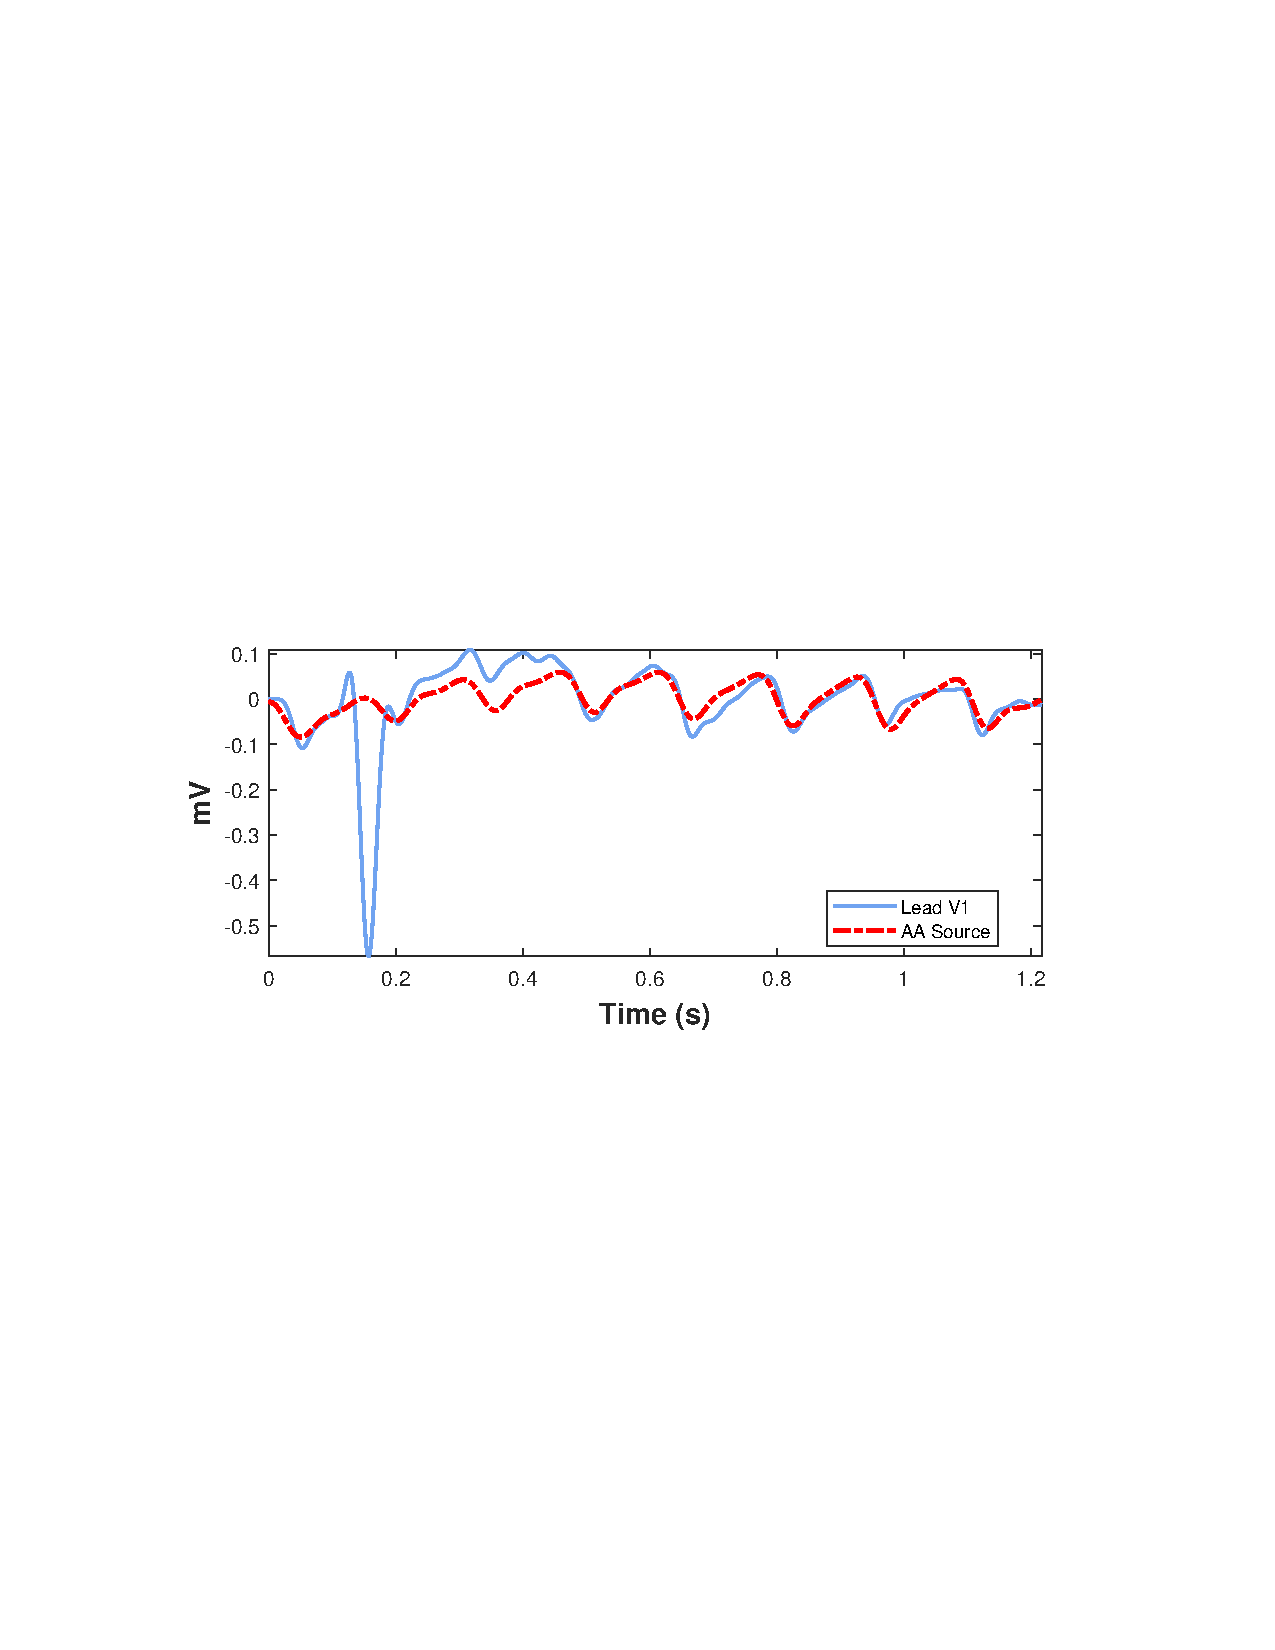
\includegraphics[scale=0.75,trim={3.0cm 8.5cm 3.0cm 8.5cm},clip=true]{figures/example_Source.pdf}
		\end{figure}
		\vspace{-2.0cm}
		
		\begin{itemize}
			\item SC $=$ 74.3\%
			\item DF $=$ 6.4 Hz
			\item Kurtosis $=$ 177.0
			\item AA Hankel Matrix Rank $=$ 33
		\end{itemize}
		
	\end{frame}

%% ------------------------- Experimental Results -----------------------------
\section{Experimental Results}

	\begin{frame}{Database and Experimental Setup} 
			
		\begin{block}{Database}
			\begin{itemize}
				\item 20 patients suffering from persistent AF
				\item 59 ECG segments from 0.72 to 1.42 seconds
			\end{itemize}
			
			\begin{center}
				Cardiology Department of Princess Grace Hospital Center, Monaco
			\end{center}					
		\end{block}	
		
		\begin{itemize}
			\item Hankel-based BTD was implemented using CAGL.
		\end{itemize}
	\end{frame}

	\begin{frame}{Impact of CA step on AA complexity}
		
		\vspace{-0.5cm}
		\begin{figure}[h]
			\centering
			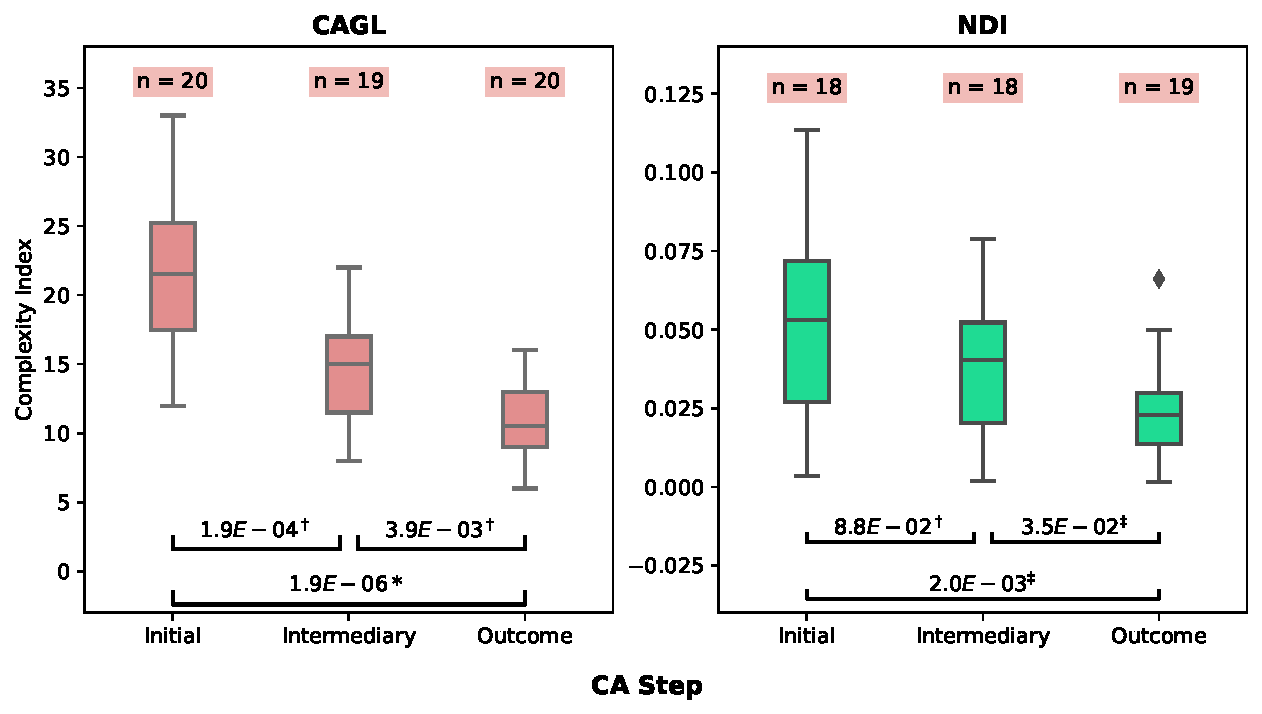
\includegraphics[scale=0.5]{figures/boxplot.pdf}
		\end{figure}
		\vspace{-0.5cm}
		\begin{itemize}
			\item 20 patients undergoing various CA steps
			\item 59 ECG segments (1.06 $\pm$ 0.2 s)
		\end{itemize}
	\end{frame}

	\begin{frame}{AF Recurrence vs. Complexity Before CA} 
		
		\vspace{-0.3cm}
		\begin{figure}[h]
			\centering
			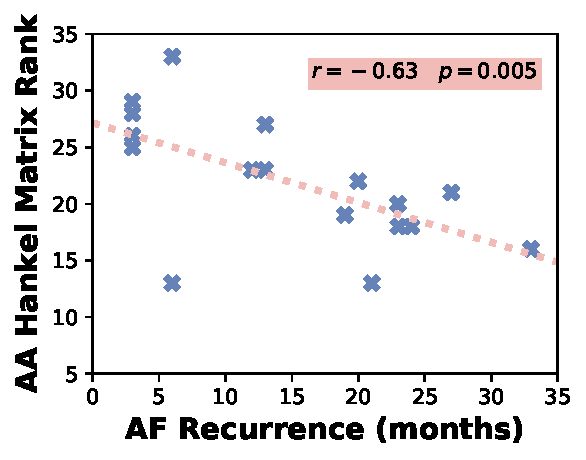
\includegraphics[scale=0.7]{figures/rank_LR.pdf}
		\end{figure}
		\vspace{-0.5cm}
		\begin{block}{Relationship}
			A significant Pearson correlation between AF recurrence and the proposed index
			\begin{itemize}
				\item 18 patients with complete follow-up information
			\end{itemize}
		\end{block}	
	\end{frame}

	\begin{frame}{AF Recurrence vs. Complexity Before CA}
		
		\begin{figure}[h]
			\centering
			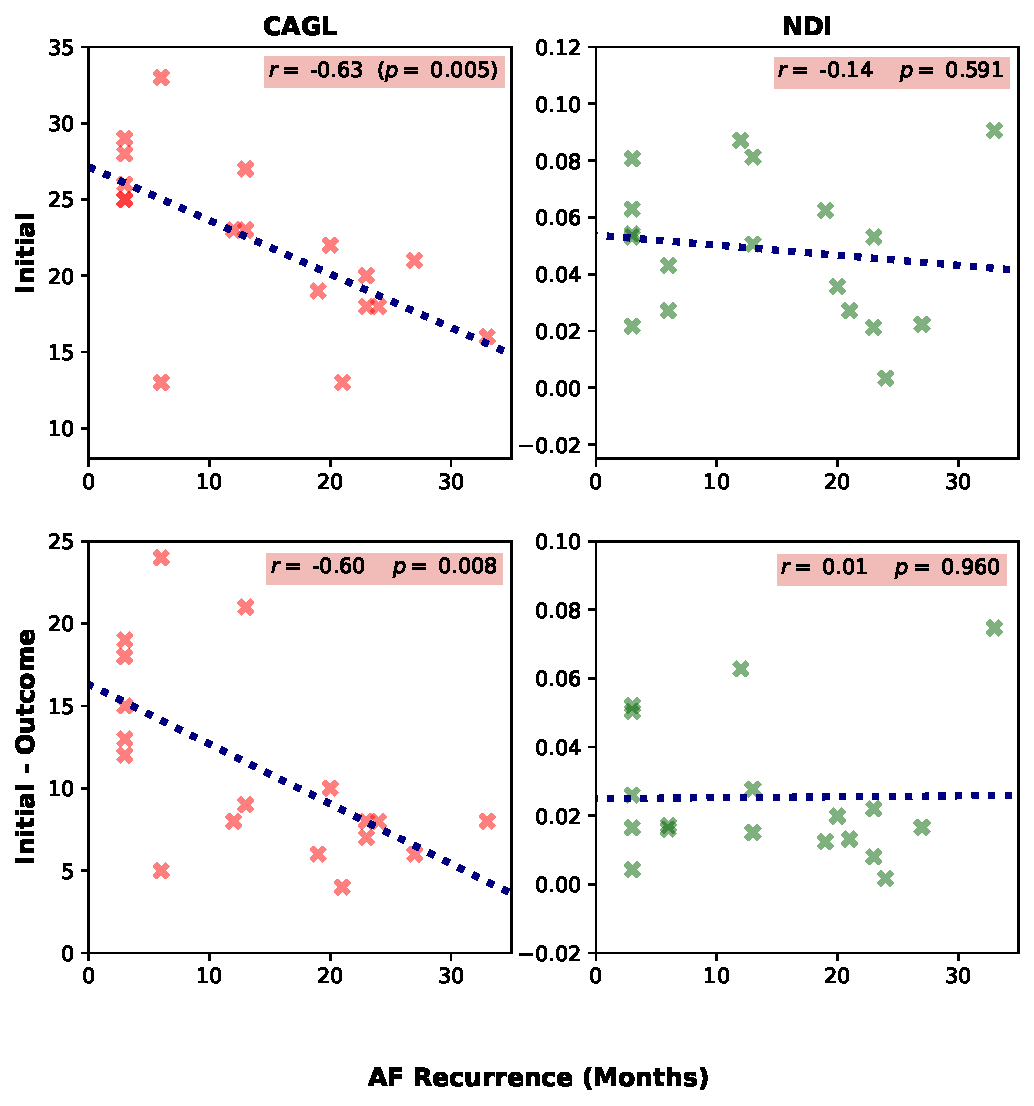
\includegraphics[scale=0.4]{figures/LR_2scenarios.pdf}
		\end{figure}
	\end{frame}

	\begin{frame}{Impact of PVI on AA complexity}

		\vspace{-0.5cm}
		\begin{figure}[h]
			\centering
			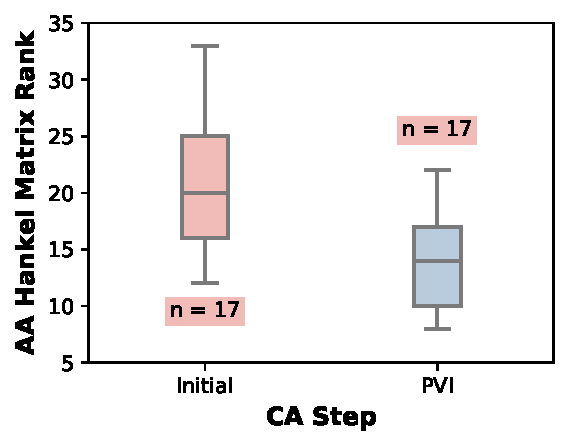
\includegraphics[scale=0.9]{figures/boxplot_PVI.pdf}
		\end{figure}
		\vspace{-0.5cm}
		\begin{itemize}
			\item 17 patients undergoing PVI
			\item 34 ECG segments
		\end{itemize}
	\end{frame}

%% ------------------------- Conclusion ---------------------------------------
\section{Conclusions}

	\begin{frame}{Conclusions} 
		
		\begin{block}{Contributions}
			\begin{itemize}
				\item Jointly extract the AA signal and measure AF complexity via tensor decomposition
				\item Very short ECG recordings (1.06 $\pm$ 0.20 s)
				\item Validation in 20 patients undergoing CA
				\begin{itemize}
					\item Expected decreasing AF complexity throughout CA steps
					\item Significant correlation with AF recurrence after CA
				\end{itemize}
			\end{itemize}
		\end{block}
		
		\begin{block}{Clinical Impact}
			\begin{itemize}
				\item A potential tool to help guide CA in real time
			\end{itemize}
		\end{block}

		\begin{block}{Future Work}
			\begin{itemize}
				\item Increase number of patients in the database
				\item Compare the proposed index with other state-of-the-art indices
				% \item Automated source classification.
			\end{itemize}
		\end{block}
		
	\end{frame}
	
	\begin{frame}{References}
		
		[1] Krijthe \textit{et al}., ``Projections on the number of individuals with atrial fibrillation in the European Union, from 2000 to 2060,'' \textit{Eur Heart J}. 2013.

		[2]	M. Meo \textit{et al}., ``Noninvasive assessment of atrial fibrillation complexity in relation to ablation characteristics and outcome,'' \textit{Frontiers in Physiology}, 2018.

		[3] De Lathauwer, ``Blind separation of exponential polynomials and the decomposition of a tensor in rank-($L_{r}$,$L_{r}$,1) terms,'' \textit{SIAM J. Matrix Anal. Appl.}, 2011.

		[4] Goulart \textit{et al}., ``Alternating group lasso for block-term tensor decomposition with application to ECG source separation'', in \textit{IEEE Transactions on Signal Processing}, vol. 68, pp. 2682-2696, 2020.
		
		[5] De Oliveira and Zarzoso, ``Source analysis and selection using block term decomposition in atrial fibrillation'', in \textit{Proc. LVA/ICA}, 2018.
	\end{frame}
	
	\begin{frame}{Previous Work}
	
		\begin{block}{CinC 2020}
			\textbf{L. S. Abdalah}, P. M. R. de Oliveira, W. Freitas Jr, and V. Zarzoso, ``Tensor-based noninvasive atrial fibrillation complexity index for  catheter ablation,'' in Proc. Computing in Cardiology, vol. 47, Rimini, Italy, Sep. 2020.
		\end{block}

		\begin{block}{SBRT 2021}
			\textbf{L. Abdalah}, W. Freitas Jr, P. M. R. de Oliveira, and V. Zarzoso, ``Low-Rank Hankel Signal Model: Numerical Results,'' in Proc. Simp\'{o}sio Brasileiro de Telecomunica\c{c}\~{o}es e Processamento de Sinais, vol. 39, Fortaleza, Brazil, Sep. 2021.
		\end{block}
	
	\end{frame}
	
	\begin{frame}{}

		\begin{center}
			Thank You!
		\end{center}
	\end{frame}

\end{document}